% DIPOLOMARBEITS TABELLEN DEUTSCH ########################
\newpage
\begin{center}
\textbf{\LARGE DIPLOMARBEIT}

\textbf{Dokumentation}
\end{center}

%Schülernamen mit Klasse oder Schuljahr
\begin{tikzpicture}
\node[da_dokubox] {
    \textcolor{darkgray}{Verfasser*innen} \\ 
    \begin{itemize} [itemsep=0pt, topsep=0pt]
        \item[] Jacob Toifl, 5AHIT
        \item[] Michael Schaider, 5AHIT
    \end{itemize}
    \textcolor{darkgray}{Abteilung} \\ 
    \begin{itemize} [itemsep=0pt, topsep=0pt]
        \item[] Informationstechnologie
        \item[] Ausbildungsschwerpunkt:
    \end{itemize}
    \textcolor{darkgray}{Schuljahr} \\ 
    \begin{itemize} [itemsep=0pt, topsep=0pt]
        \item[] 2025/2026
    \end{itemize}
        \textcolor{darkgray}{Thema der Diplomarbeit} \\ 
    \begin{itemize} [itemsep=0pt, topsep=0pt]
        \item[] DropIT - strukturierte digitale Dokumentenablage
    \end{itemize}
        \textcolor{darkgray}{Kooperationspartner} \\ 
    \begin{itemize} [itemsep=0pt, topsep=0pt]
        \item[] MBIT Solutions GmbH
    \end{itemize}
}; %node (Rahmen)
\end{tikzpicture}

\vspace{0.5cm}

\begin{tikzpicture}
\node[da_dokubox] {
    \textcolor{darkgray}{Aufgabenstellung} \\ 
In vielen Unternehmen fehlt eine einheitliche und strukturierte digitale Dokumentenablage. Verträge und Unterlagen werden unsystematisch gespeichert, wodurch klare Zugriffsrechte fehlen und wichtige Informationen schwer auffindbar sind. Dies führt zu Fristversäumnissen, erhöhtem Suchaufwand, Fehlern und Sicherheitsrisiken.
Ziel dieser Diplomarbeit ist die Entwicklung von DropIT – einer zentralen, benutzerfreundlichen Dokumentenablage mit KI-gestützter Klassifizierung. Das System soll Dokumente automatisch erkennen und kategorisieren, eine schnelle Suche ermöglichen und über ein Erinnerungssystem vor Fristversäumnissen schützen. Die Integration erfolgt über Microsoft SharePoint und Entra ID.
    }; %node (Rahmen)
\end{tikzpicture}

\vspace{0.5cm}

\begin{tikzpicture}
\node[da_dokubox] {
    \textcolor{darkgray}{Realisierung} \\ 
Das System wurde als moderne Webanwendung entwickelt, bei der sich Benutzer mit ihrem bestehenden Microsoft-Firmenkonto anmelden können. Dokumente werden automatisch in der vorhandenen SharePoint-Umgebung des Unternehmens gespeichert, sodass keine separate Datenhaltung erforderlich ist.
Ein zentrales Element ist die intelligente Dokumentenerkennung: Beim Hochladen analysiert das System automatisch den Inhalt und erkennt, um welchen Dokumententyp es sich handelt – etwa einen Vertrag, eine Rechnung oder ein Angebot. Relevante Informationen wie Ablaufdaten oder Kundennamen werden dabei automatisch ausgelesen.
Die Anwendung ist so aufgebaut, dass sie problemlos mit steigenden Anforderungen wachsen kann und sich flexibel erweitern lässt.
    }; %node (Rahmen)
\end{tikzpicture}

\vspace{0.5cm}

\begin{tikzpicture}
\node[da_dokubox] {
    \textcolor{darkgray}{Ergebnisse} \\ 
Im Rahmen dieser Diplomarbeit wurde eine voll funktionsfähige Dokumentenverwaltung entwickelt. Benutzer können sich über ihr bestehendes Microsoft-Konto anmelden und erhalten automatisch die entsprechenden Berechtigungen.
Das Herzstück der Anwendung ist die KI-gestützte Dokumentenerkennung, die hochgeladene Dateien automatisch klassifiziert und relevante Metadaten wie Ablaufdaten oder Vertragspartner extrahiert. Dokumente können per Drag \& Drop in frei definierbare Upload-Zonen abgelegt werden, wobei die Ablage direkt in SharePoint erfolgt.
Die implementierte Volltextsuche ermöglicht ein schnelles Auffinden von Dokumenten nach Schlagworten, Dokumententyp oder Datum. Zusätzlich können Dokumente direkt in der Anwendung in einer Vorschau angezeigt und heruntergeladen werden.
Das integrierte Erinnerungssystem benachrichtigt Benutzer rechtzeitig über ablaufende Fristen und anstehende Aufgaben, wodurch Fristversäumnisse vermieden werden.
\begin{center}
 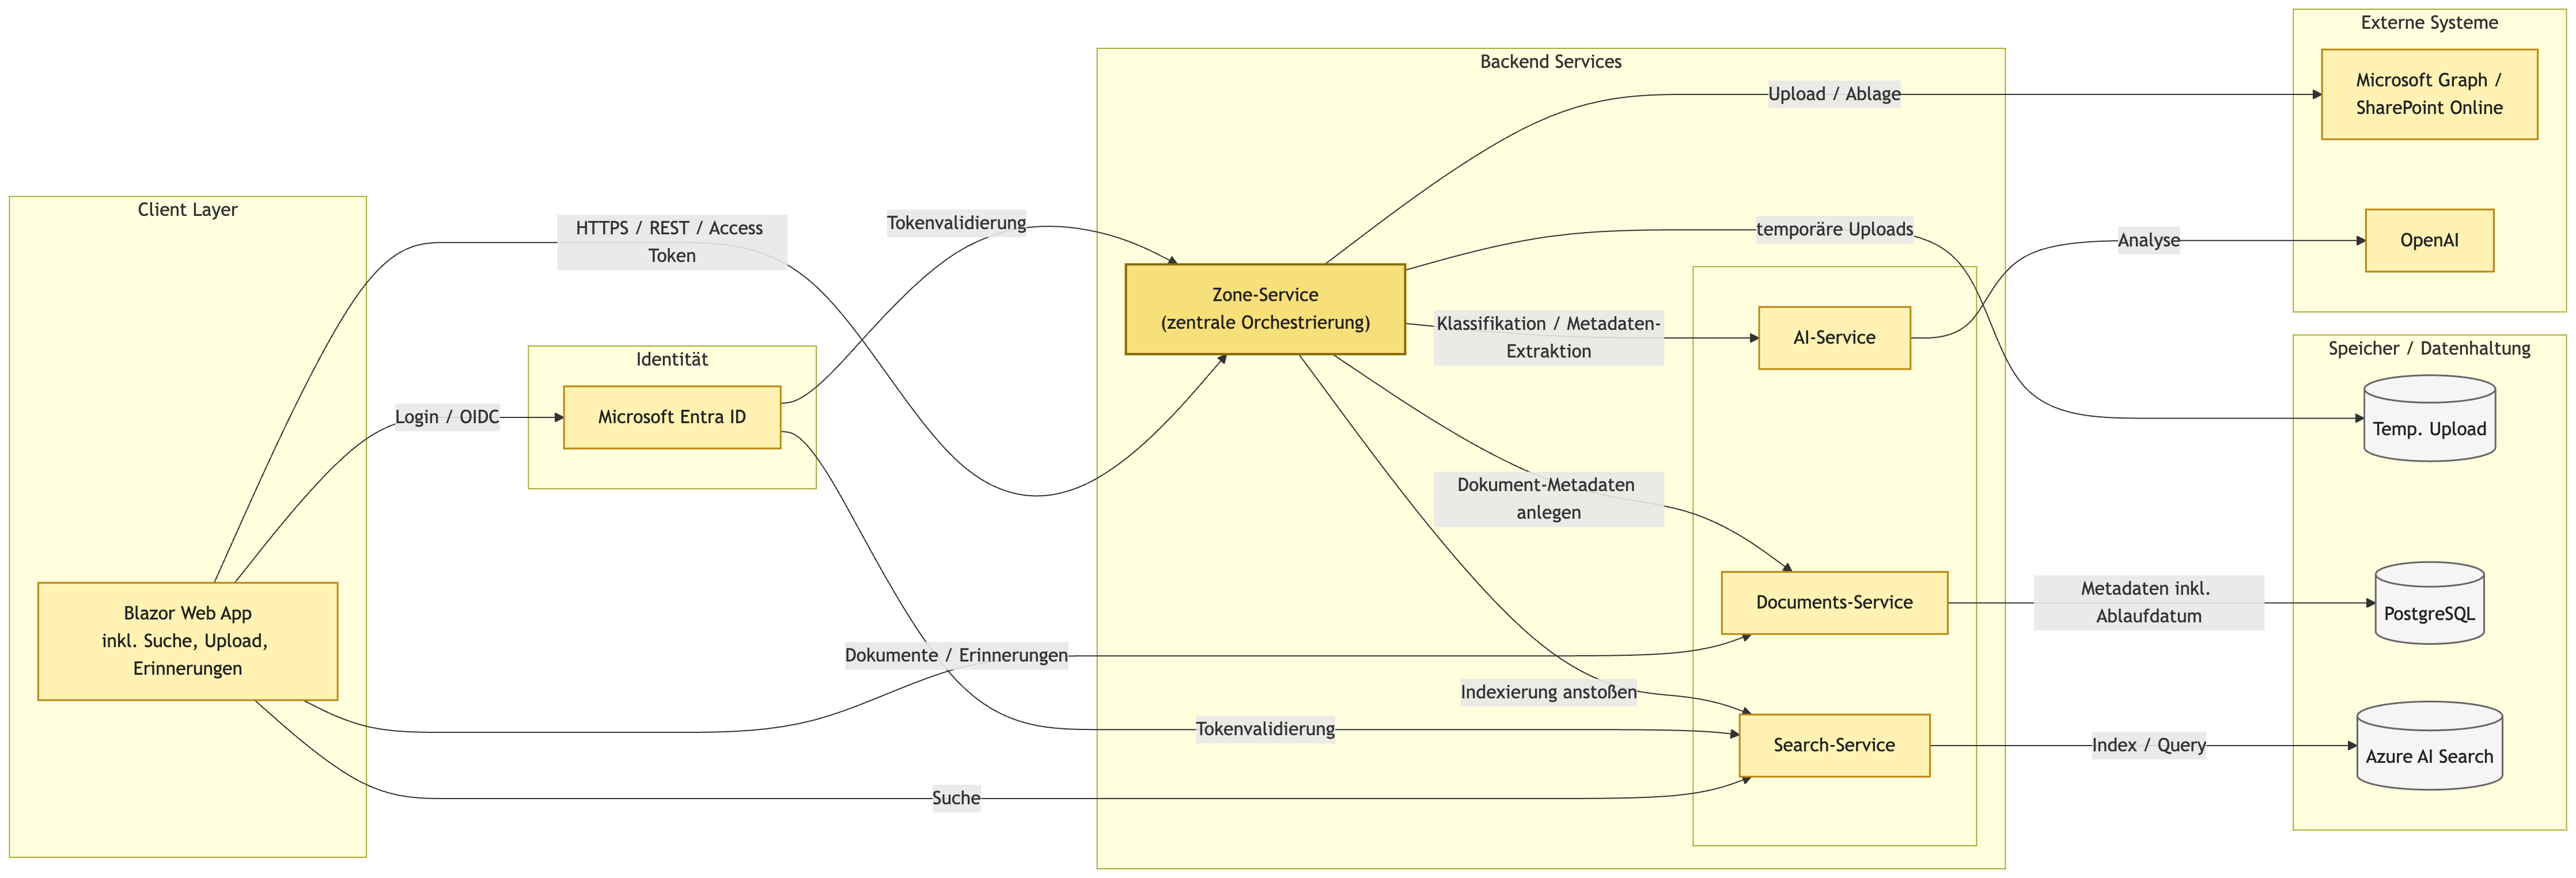
\includegraphics[width=0.95\textwidth]{content/img/4_deployment/systemarchitektur.png}
\end{center}

}; %node (Rahmen)
\end{tikzpicture}